% ------------ NEW CHAPTER ------------
\chapter{Návrh riešenia}
Kapitola bude zahŕnať použitý software pre tvorbu klasifikátorov a neurónových sieti, špecifikáciu hardwaru na ktorom bude trénovanie priebiehať.
Ďalej priblíži zbroje a spôsoby pre získanie, spracovanie a rozdelenie dát zbraní určených pre klasifikáciu typu a určenie náklonu v scéne.
Následne opíše celkový navrhovaný postup, od predspracovania obrazu až po zber výsledkov.
Celá kapitola bude vychádzať z informácií ktoré boli spomenuté v kapitole \ref{chap:technologie}.



\section{Použitý software a hardware}
\label{sec:softwarehardware}
Prvým bodom pri návrhu riešenia je dôležité vybrať správny programovací jazyk a nástroje, ktoré sú pre riešenie daného problému vhodné
    a ktoré môžu uľahčiť aj celkovú implementáciu.

V kapitole \ref{sec:frameworks} bol vytvorený základny prehľad populárnych nástrojov pre tvorbu klasifikátorov, neurónových sietí a predspracovanie obrazu.
Vzhľadom na porovnanie týchto nástrojov, bude pre túto prácu použitý programovací jazyk Python, knižnica Keras pre tvorbu konvolučných neurónových sietí, ktorá
    ako svoj backend bude využívať knižnicu TensorFlow.
A následne pre klasický prístup ku klasifikácií obrázkov bude použitá knižnica Scikit-learn a Scikit-image pre implementáciu predspracovania obrazu.

Keďže trénovanie klasifikátorov a neurónových sietí je výpočetne náročna operácia, je vhodné použiť výkonný hardware a akceleráciu výpočtou na GPU.
Pre túto prácu bude použitý počitač so štvorjadrovím procesorom i7-6700HQ, veľkosťou operačnej pamäte 16 GB a grafickou kartou Nvidia GeForce 940MX.
Na použitom počitači bude nainštalovaný 64-bitový operačný systém Fedora 27.



\section{Klasifikácia typu zbrane}
\label{sec:klasfikaciatypuzbrane}
Jedným z cieľov tejto práce je klasifikovať typy zbraní do 2 kategórií, a to na krátke a dlhé zbrane.
Táto klasifikácia môže prebiehať niekoľkými spôsobmi, prehľad týchto prístupov bol zhrnutý v kapitolách \ref{sec:detekcia} a \ref{sec:klasifikacia}.
Pre klasifikáciu v tejto práci bude použitých niekoľko z týchto prístupov a vo výsledku budú porovnané, ktorý dosiahol najlepšie výsledky.

Prvé riešenie bude spočívať v klasickom prístupe, ktoré pozostáva z predspracovania vstupných dát pomocou prekonvertovania dát do šedotónového obrazu a histogramu orientovaných prechodov (viď. \ref{sec:preprocessing}).
Na tieto predspracované dáta bude v jednom z riešení použitý K-Nearest-Neighbor klasfikátor, pre druhé riešenie bude použitý SVM klasifikátor, testovanie
    a porovnávanie výsledkov môže prebiehať s rôznymi konfiguráciami týchto klasifikátorov.
\begin{enumerate}
    \item[$\bullet$] Pre \textbf{K-Nearest-Neighbor}, knižnica scikit-learn poskytuje 2 rôzne implementácie tohto klasifikátora.
    Trieda \textit{KNeighborsClassifier} klasifikuje na základe $k$ najbližších susedov, kde $k$ je celé číslo špecifikované užívateľom.
    
    Druhá implementácia je trieda \textit{RadiusNeighborsClassifier}, ktorá klasifikuje na základe počtu susedov v rámci pevného polomeru $r$ každého trénovacieho bodu,
        kde $r$ je hodnota s pohyblivou desatinnou čiarkou určená užívateľom\footnote{\url{http://scikit-learn.org/stable/modules/neighbors.html\#nearest-neighbors-classification}}.
    \item[$\bullet$] Pre \textbf{Support Vector Machines}, scikit-learn obsahuje 3 triedy \textit{SVC}, \textit{NuSVC} a \textit{LinearSVC} pre viac-triednu
        klasifikáciu s možnosťou použitia rôznych typov jadier \footnote{\url{http://scikit-learn.org/stable/modules/svm.html\#custom-kernels}}.
    %\item[$\bullet$] \textbf{Multi Layer Perceptron}
\end{enumerate}

Pre dalšie riešenie klasfikácie zbraní budú použité dve konvolučné neurónové siete, ktorých výsledky budú porovnané, všeobecná architektúra sietí je opísana v kapitole \ref{sec:architekuraCNN}.
Výsledok poslednej vrstvy softmax klasfikatóra budú 2 výstupy, ktoré budú určovať typ zbrane.
Predspracovanie vstupných dát bude pozostávať z normalizacie hôdnot RGB zložiek pixelov, nastavenia rovnomernej veľkosti strán obrázka (viď. \ref{sec:preprocessing})
    a následnej augmentácií dát pre zväčsenie počtu vstupných dát (viď. \ref{subsec:augmentacia}).



\section{Určenie náklonu zbrane}
Druhý z cieľou tejto práce je určenie náklonu zbrane v obraze.
Tento náklon bude určeny v 3 osách.
Dôležité je spomenúť že názvy ós sú pomenované podľa tých ktoré sa používajú v letectve, vid. obrázok \ref{pic:airplaneaxis}.
\begin{figure}[H]
    \centering
    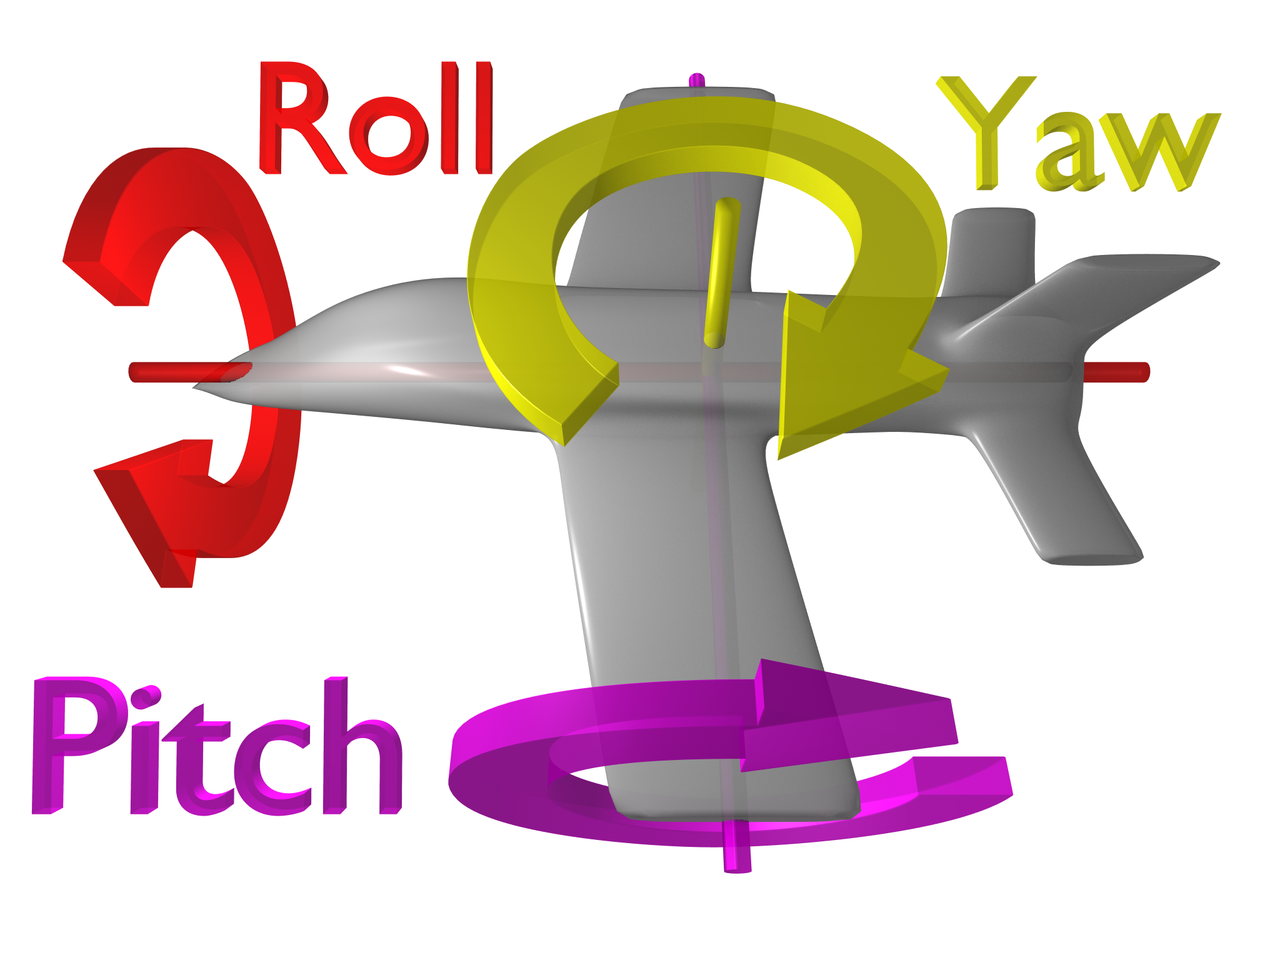
\includegraphics[width=0.5\textwidth]{airplane-axis}
    \caption{Mená ós pre letectvo.}
    \label{pic:airplaneaxis}
\end{figure}

Tento problém je môžné preniesť do klasifikácie, preto pre riešenie tohto problému budú použité konvolučné neurónové siete, ktorých všeobecná architektúra je popísana v \ref{sec:architekuraCNN}.
Výsledok poslednej vrtsvy softmax klasfikátora bude 72 výstupov ktoré budú určovať o aký uhol je zbraň natočená.
Každá zo 72 kategórií bude zastupovať rozpätie 5 stupňov, ciže celkovo sa určí náklon zbrane v celom rozsahu od 0 do 360 stupňov.

Postup predspracovania obrazu bude rovnaký ako pri klasfikácií zbraní pomocou konvolučných neurónových sieti, normalizácia, úprava rozmeru vstupu na štvorec a augmentácia dát (vid. \ref{subsec:augmentacia})
Pre každú os bude natrénovaná samostatná konvolučná neurónová sieť, výsledok bude teda obsahovať 3 natrénované modely.

\subsection{Odchylka chyby}
Knižnica Keras obsahuje funkciu \textit{categorical\_accuracy}\footnote{\url{https://keras.io/metrics/}} pre určenie presnosti siete pri klasfikovaní do viacerých kategórií.
Čo je možné použiť, avšak pre určenie náklonu by bola vhodná iná metrika určovania presnosti siete.
Preto bude implementovaná vlastná funkcia \textit{angle\_error} ktorá bude počitať presnosť siete podľa priemerného rozdielu medzi skutočnými a predpovedanými uhlami.



\section{Konvolučné neurónové siete}
\label{sec:architekuraCNN}

\subsection{Nastavenie parametrov}
\label{subsec:nastavenieparametrov}
Ako bolo spomínané v kapitole \ref{subsec:convolutionalneuralnetwork} je niekoľko parametrov, ktoré je potrebné
    nastaviť v konvolučných a pooling vrstvách.
Pre správne fungovanie siete je potrebné nastaviť aj správne hodnoty týchto parametrov, preto v navrhovaných architektúrach budú
    hodnoty parametrov nastavené na tie najpoužívanejšie.

Veľkosť výstupu a správnosť nastavenia parametrov v konvolučnej vrstve je možné výpočítať pomocou vzťahu:
\begin{equation}
    \frac{(W - F + 2*P)}{S} + 1
\end{equation}
Kde $W$ je veľkosť vstupných dát, $F$ je veľkosť filtra, $P$ je nastavenie zarovnania, v prípade nulového zarovnania je hodnota 1 a $S$ je veľkosť kroku.
Pre správné nastavenie musí byť výsledná hodnota celé číslo, kde táto výsledná hodnota udáva aj veľkosť výstupu.
Najpoužívanejšie hodnoty parametrov sú: $F = 3, S = 1, P = 1$ a vstup $W$ o hodnote, ktorá je deliteľná číslom 2 \cite{odkaz:CNNArchitecture}.

Funkciou pooling vrstvy je znižovanie dimenzionality a zároveň ponechanie dôležitých informácií, ako najpoužívanejšie hodnoty parametrov sú
    veľkosť filtra 2x2 s krokom 2 pri použití MaxPooling vrstvy \cite{odkaz:CNNArchitecture}.

% TODO batch-size, epochy
% CNN sa trenuje v cykloch nazyvanych epochy, v kazdej epoche prejdu cez sieť vsetky obrazky na ktorych sa sieť uci,
% pre ucenie je potrebne zvolit vhodny pocet tychro epoch aby sieť podala najelpsie vysledky a zaroven sa nepretrenovala.
% Preto je vhodne ukoncit trenovanie v bode kedy klesa presnosť siete na validacnych datach, v takom pripade to moze vies k pretrénovaniu siete
% na trenovacich datach.

\subsection{Návrh architektúr}
\label{subsec:navrharchitektur}
Prvý model siete je inšpirovaný architektúrou AlexNet (viď. \ref{subsec:popularCNN}).
Model obsahuje celkovo 20 vrstiev, z ktorých 5 je konvolučných, 5 max pooling, 7 dropout a 3 dense vrstvy.
Veľkosť vstupných dát do prvej vrstvy je 128x128x3.
Vo všetkých konvolučných vrstvách sú použité filtre o veľkosti 3x3 s krokom 1 a použitím nulového zarovnania.

V modeli sa každou konvolučnou vrstvou zdvojnásobuje počet filtrov, z počiatočných 16 až na 256 v poslednej vrstve.
Pooling vrstvy sú typu max, veľkosť filtra je 2x2 s posunom 2 po každej osi.
Za každou pooling vrstvou sa nachádza Droupout vrstva s nastavením 0.2, čiže 20 percent náhodných prepojení sa ignoruje.

Po piatich blokoch konvolučnej, pooling a droupout vrstvy nasledujú 2 dense vrstvy s počtom prepojení 1024 a dropout vrstvou s nastavním 0.5.
Ako posledná je dense vrstva s 2 alebo 72 prepojeniami a softmax klasifikátorom, počet výstupov závísí od toho, či určujeme typ alebo náklon zbrane.
V celej sietí sú použité ReLu aktivačné funkcie.

\begin{figure}[H]
    \centering
    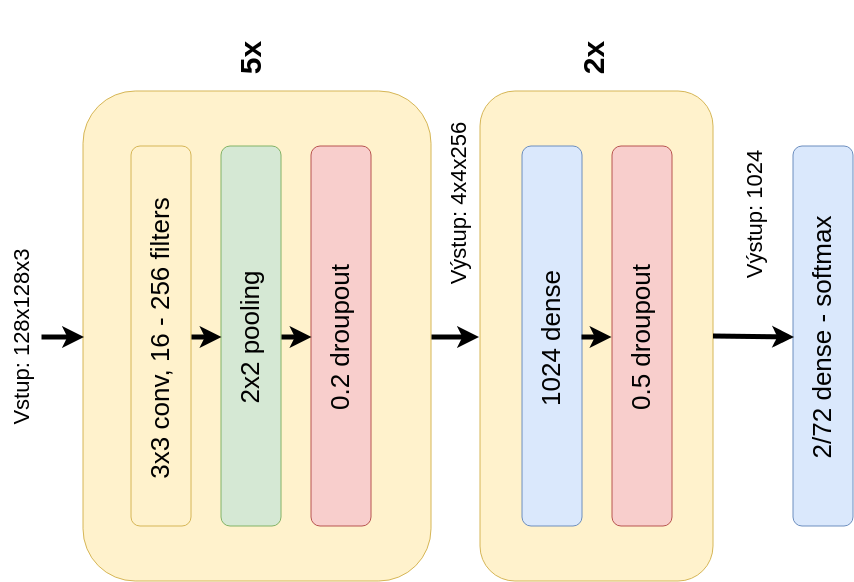
\includegraphics[width=0.6\textwidth]{AlexNet_Like}
    \caption{AlexNet-Like navrhovaná architektúra.}
    \label{pic:kNN}
\end{figure}

% ----------- DRUHY NAVRH -----------

Druhý navrhovaný model je inšpirovaný architektúrou VGG sietí (viď. \ref{subsec:popularCNN}).
Vzhľadom na možnosti výkonu na ktorom bude trénovanie prebiehať, je navrhovaná sieť o dva bloky vrstviev menšia a taktiež konvolučne vrstvy obsahujú menej filtrov.

Celkovo sieť obsahuje 2 bloky obsahujúce 2 konvolučné vrstvy s počtom filtrov 32 a 64, pooling a droupout vrstvu s 20\% ignorovaním prepojení.
Ďalej nasledujú 3 konvolučné vrstvy so 128 filtrami a pooling vrstva.
Ako posledné sú 2 bloky obsahujúce dense vrstvu s počtom prepojení 2048 a dropout vrstvu s ignorovaním nastaveným na 50\%.
Posledná výstupná vrstva obsahuje 2 alebo 72 prepojení so softmax klasfikátorom.
Každá konvolučná vrstva obsahuje filtre o veľkosti 3x3, krokom 1 a s použitím nulového doplnku.
Pooling vrstvy sú typu max, veľkosť filtra je 2x2 s posunom 2 po každej osi.
V celej sietí je použitá ReLu aktivačná funkcia.

\begin{figure}[H]
    \centering
    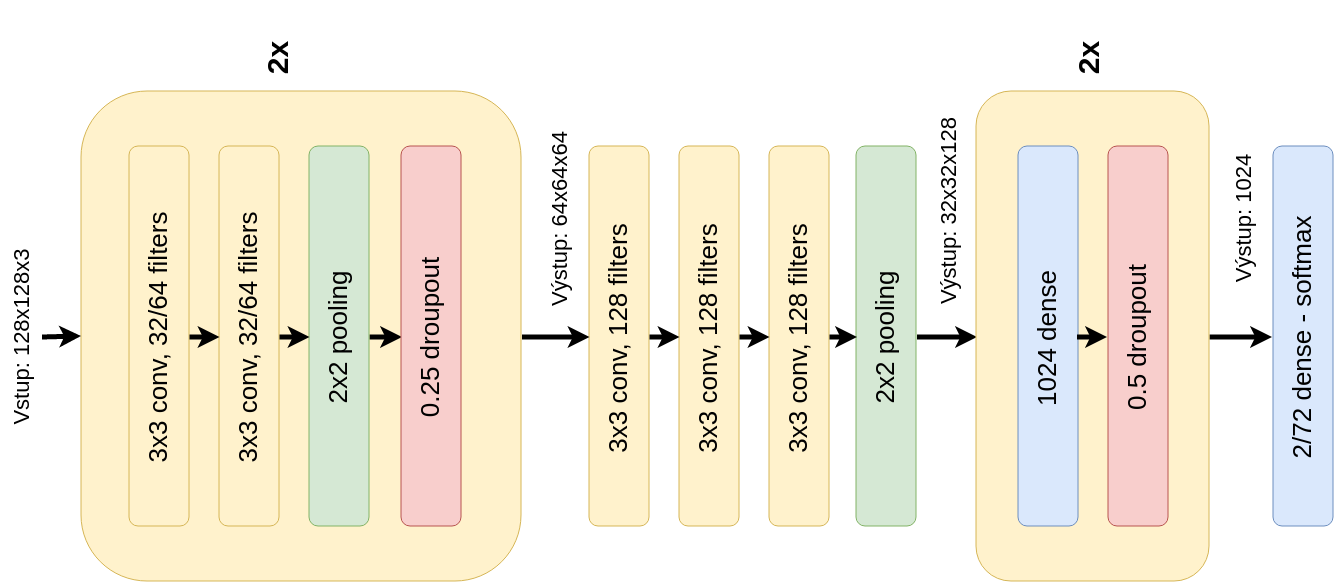
\includegraphics[width=0.8\textwidth]{VGG_Like}
    \caption{VGG-Like navrhovaná architektúra.}
    \label{pic:kNN}
\end{figure}



\section{Trénovacia databáza zbraní}
\label{sec:databaza}
Pre správne trénovanie klasifikátorov a neurónových sietí je dôležité mať dáta v dostatočnom počte a správne označené.
Trénovacia databáza je získana z niekoľkých zdrojov.
\begin{enumerate}
    \item[$\bullet$] \textbf{IMFDB}\footnote{\url{http://www.imfdb.org/wiki/Main_Page}} - je databáza záberov z filmov v ktorých sa nachádzajú zbrane.
    Obsahuje nie len celkové scény ale aj samostatné obrázky zbraní ktoré sa v danej scéne nachádzajú.
    Pre túto prácu je potrebné aby daný obrázok obsahoval iba zbraň, preto je potrebné obrázky z tejto databázy ručne odfiltrovať na samotné zbrane a scény so zbranami.
    Následne ich potom zaradiť do správnej kategórie na krátke a dlhé.
    \item[$\bullet$] \textbf{ImageNet}\footnote{\url{http://www.image-net.org/}} - je databáza obrázkov ktorá obsahuje viac ako 14 miliónov obrázkov vo viac ako 21000 kategóriach.
    Výhodou tejto databázy je, že obrázky už patria do určenej kategórie a tak nieje potrebné ich ručné prechádzať a kategorizovať.
    \item[$\bullet$] \textbf{Google}\footnote{\url{http://www.google.com}} - pre doplnanie a zväčšenie počtu obrázkou je môžné použiť google vyhľadávanie.
    Tak ako v prípade IMFDB bude potrebné obrázky ručne kategorizovať.
    \item[$\bullet$] \textbf{Free3D}\footnote{\url{https://free3d.com/3d-models/weapons}} - databáza voľne dostupných 3D modelov zbraní s textúrami v rôzných formátoch.
\end{enumerate}

Databáza zbraní z prvých 3 zdrojov je možné použiť na klasficikáciu zbraní do 2 kategórií na krátke a dlhé zbrane.
Pre trénovanie neurónových sietí na určenie náklonu zbrane v obraze bude potrebné použiť 3D modely zbraní a následne pomocou nich vygenerovať
    obrázky zbraní v požadovaných natočeniach zbrane v obraze.

\subsection{Generovanie dát z 3D modelov}
\label{subsec:generovanie3d}
Generovanie obrázkov pre určenie náklonu zbrane v scéne bude prebiehať pomocou databázy 3D modelov zo zdroja Free3D.
Následne sa použije software od Ing. Tomáša Goldmanna na generovanie obrázkov z 3D modelov\footnote{\url{http://www.fit.vutbr.cz/~igoldmann/app/SYDAGenerator}},
    do ktorého je potrebné vložiť 3D model vo formáte g3db a pozadie scény.

Keďže 3D modely ktoré budú použité niesu v požadovanom formáte, je potrebné ich prekonvertovať, to je môžné urobiť
    pomocou nástroja \textbf{fbx-conv}\footnote{\url{https://github.com/libgdx/fbx-conv}}.
Tento nástroj podporuje konvertovanie 3D modelov z formátu fbx alebo obj do požadovaného formátu g3db.

\subsection{Augmentácia obrázkov}
\label{subsec:augmentacia}
Ako bolo opísane v kapitole \ref{sec:preprocessing} jedna z možností zväčšenia počtu vstupných dát a zlepšenia generalizácie pri klasifikácií je augmentácia vstupných dát.
V tejto práci môžeme rozdeliť augmentáciu dát do dvoch skupín, prvý druh augmentácie bude prebiehať pre trénovanie klasifikátorov ktoré
    určuju typ zbrane, druhý druh augmentácie bude prebiehať pri obrázkoch určených pre náklon zbrane.

Pri augmentácií dát pre klasifikovanie dvoch tried, na krátke a dlhé zbrane, prebehne niekoľko transfomácií obrázka.
\begin{enumerate}
    %\item[$\bullet$] \textbf{priblíženie} - priblíženie alebo oddialenie vstupného obrázku
    \item[$\bullet$] \textbf{Rotácia} - obrázky budú rotované o náhodny uhol v rozmedzí 0-180 stupňov.
    \item[$\bullet$] \textbf{Preklopenie} - vertikálne alebo horizonálne preklopenie obrázka.
    \item[$\bullet$] \textbf{Posun} - posun obrázka po x-ovej a y-ovej osi.
    \item[$\bullet$] \textbf{Výplň} - pri rotácií alebo posunu obrázku môže vzniknúť čierna plocha pixelov, tieto čierne pixely je potrebné vyplniť.
    Tieto čierne pixely budú doplnené hraničným pixelom obrázka ktorý bude nakopírovaný až po nový okraj.
\end{enumerate}

\begin{figure}[H]
    \centering
    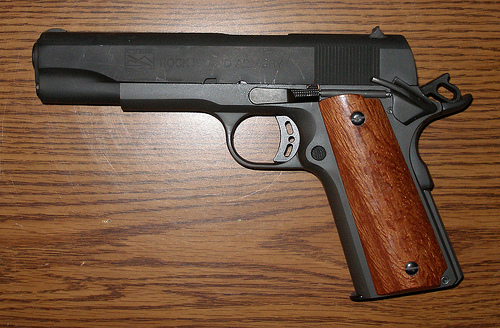
\includegraphics[width=0.4\textwidth]{weapons/weapon}
    \qquad
    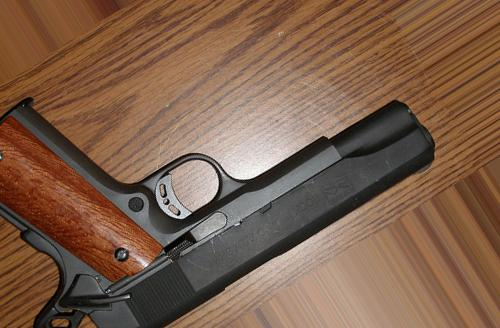
\includegraphics[width=0.4\textwidth]{weapons/weapon-augmented}
    \caption{Pôvodny obrázok (vľavo), augmentovaný obrázok (vpravo)}
    \label{pic:imageAugmented}
\end{figure}

Druhý typ augmentácie dát prebieha pri obrázkoch ktoré boli vygenerované pomocou 3D modelu.
Keďže nieje potrebné generovať všetky polohy otočenia od 0 po 360 stupňov, stačí vygenerovať dáta v polohách od 0 po 90 stupňov a od 270 do 359 stupňov
    zvyšné polohy je možné dogenerovať pomocou transformácie obrázka, pomocou vertikálneho alebo horizonálneho preklopenia.
Avšak v tomto prípade je potrebné po transformácií obrázka vyrátať novú hodnotu uhla transformovaného obrázka, to je môžené dosiahnuť pomocou niekoľkých
    jednoduchých vzorcov.

\textbf{Roll}, pri natočení modelu v ose roll, je potrebné aplikovať horizontálne preklopenie obrázka.
Následne uhol transformovaného obrázka $trans\_angle$ bude vypočítaný z pôvodneho uhla $angle$ podľa:
\begin{equation}
    trans\_angle = -angle + 540 \quad ak \; 270 \leq angle \leq 359
\end{equation}
\begin{equation}
    trans\_angle = abs(angle - 180) \quad ak \; 0 \leq angle \leq 90
\end{equation}

\begin{figure}[H]
    \centering
    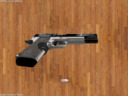
\includegraphics[width=0.3\textwidth]{weapons/roll_300}
    \quad
    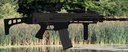
\includegraphics[width=0.3\textwidth]{weapons/roll_0}
    \quad
    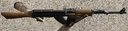
\includegraphics[width=0.3\textwidth]{weapons/roll_70}
    \caption{Natočenie zbrane v ose roll, 300 stupňov(vľavo), 0 stupňov(v strede), 70 stupňov(vpravo)}
    \label{pic:rollrotation}
\end{figure}

\textbf{Yaw}, pri natočení v ose yaw, sa aplikuje vertikálne preklopenia obrázka.
Uhol transformovaného obrázka sa vypočít podľa:
\begin{equation}
    trans\_angle = abs(angle - 540) \quad ak \; 270 \leq angle \leq 359
\end{equation}
\begin{equation}
    trans\_angle = abs(angle - 180) \quad ak \; 0 \leq angle \leq 90
\end{equation}

\begin{figure}[H]
    \centering
    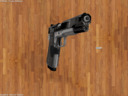
\includegraphics[width=0.3\textwidth]{weapons/yaw_300}
    \quad
    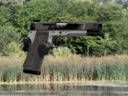
\includegraphics[width=0.3\textwidth]{weapons/yaw_0}
    \quad
    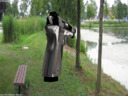
\includegraphics[width=0.3\textwidth]{weapons/yaw_75}
    \caption{Natočenie zbrane v ose yaw, 300 stupňov(vľavo), 0 stupňov(v strede), 75 stupňov(vpravo)}
    \label{pic:yawrotation}
\end{figure}

\textbf{Pitch}, v ose pitch postačuje vygenerovať obrázok zbrane s náklonom 0 stupňov so smerovaním hlavne zbrane doprava.
Počas augmentácie dát sa môže aplikovať horizontálne preklopenie a následne sa tento vstupný obrázok otočí o náhodny uhol.
Preto nieje potrebný žiaden další prepočet uhla.

\begin{figure}[H]
    \centering
    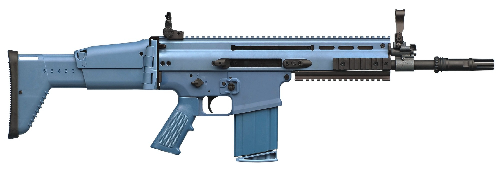
\includegraphics[width=0.3\textwidth]{weapons/pitch_0}
    \quad
    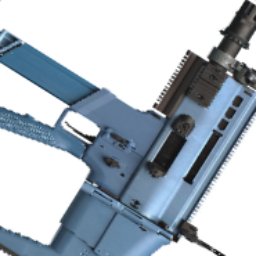
\includegraphics[width=0.2\textwidth]{weapons/pitch_60}
    \quad
    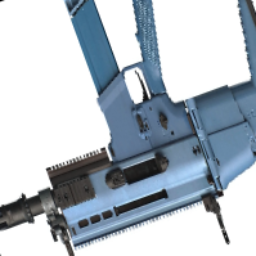
\includegraphics[width=0.2\textwidth]{weapons/pitch_200}
    \caption{Natočenie zbrane v ose pitch, 0 stupňov(vľavo), 60 stupňov(v strede), 200 stupňov(vpravo)}
    \label{pic:yawrotation}
\end{figure}



\section{Zhrnutie kapitoly}

Kapitola zhrnula software ktorý sa bude používať pre tvorbu a trénovanie klasfikátorov a neurónových sieti.
Taktiež obsahuje popis parametrov zariadenia na ktorom toto trénovanie bude prebiehať.

Následne v kapitole \ref{sec:klasfikaciatypuzbrane} je opísaný navrhovaný spôsob pre klasifikáciu typu zbrane do 2 tried, na krátku a dlhú, približuje
    programové triedy ktoré je možné pre tento problém použiť z knižnice scikit-learn.
A predstavuje celkový postup klasfikácie od predspracovania obrazu až po konečný výsledok.

Kapitola \ref{sec:urcenienaklonuzbrane} opisuje navrhovaný postup riešenia pre určenie typu zbrane pomocou konvolučných neurónových sieti,
    vysvetľuje terminológiu pre použité názvy ós rotácie a v \ref{subsec:odchylkachyby} približuje navrhovanú funkciu pre lepšie určenie presnosti siete
    pri určovaní náklonu zbrane.

Celá kapitola \ref{sec:architekuraCNN} je venová podrobnému opisu dvoch navrhovaných architektúr konvolučných neurónových sieti a
    vysvetleniu všetkých zvolených hodnôt parametrov siete.

V závere su spomenuté zdroje z ktorých je možné čerpať obrázky a 3D modely zbraní, je opísany postup generovanie obrázkov z 3D modelov a ich úprava
    pre účely tejto práce.
Posledná podkapitola \ref{subsec:augmentacia} obsahuje zoznam transformácií obrazu pre augmentáciu dát.
Opisuje 2 druhy augmentácie použitých v tejto práci, kde prvý je zameraný na dáta určené pre klasifikáciu zbraní do 2 tried a druhý pre dáta
    určené na stanovenie náklonu zbrane v obraze.
